\documentclass[tikz, border=10pt]{standalone}
\usepackage{tikz}

\begin{document}
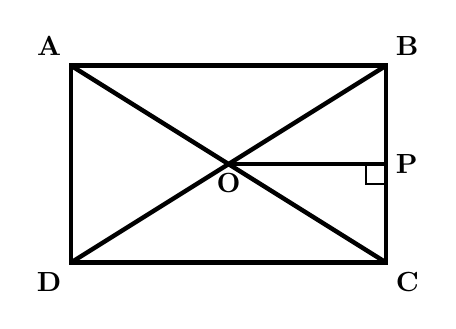
\begin{tikzpicture}

% Define rectangle vertices
\coordinate (A) at (0, 2.5);
\coordinate (B) at (4, 2.5);
\coordinate (C) at (4, 0);
\coordinate (D) at (0, 0);

% O is the center (intersection of diagonals)
\coordinate (O) at (2, 1.25);

% P is on BC (right side)
\coordinate (P) at (4, 1.25);

% Draw the rectangle ABCD
\draw[ultra thick] (A) -- (B) -- (C) -- (D) -- cycle;

% Draw diagonal AC
\draw[ultra thick] (A) -- (C);

% Draw diagonal DB
\draw[ultra thick] (D) -- (B);

% Draw line OP
\draw[ultra thick] (O) -- (P);

% Draw right angle mark at P
\def\sq{0.25}
\draw[thick] (P) ++(-\sq, 0) -- ++(-0, -\sq) -- ++(\sq, 0);

% Labels
\node[above left] at (A) {\textbf{A}};
\node[above right] at (B) {\textbf{B}};
\node[below right] at (C) {\textbf{C}};
\node[below left] at (D) {\textbf{D}};
\node[below] at (O) {\textbf{O}};
\node[right] at (P) {\textbf{P}};

\end{tikzpicture}
\end{document}